\documentclass[12pt,a4paper]{article}

% Packages
\usepackage[utf8]{inputenc}
\usepackage[T1]{fontenc}
\usepackage{lmodern}
\usepackage[margin=2.5cm]{geometry}
\usepackage{setspace}
\usepackage{booktabs}
\usepackage{tabularx}
\usepackage{graphicx}
\usepackage{amsmath}
\usepackage{amssymb}
\usepackage{natbib}
\usepackage{hyperref}
\usepackage{float}
\usepackage{caption}
\usepackage{subcaption}
\usepackage{microtype}
\usepackage{parskip}

\hypersetup{
    colorlinks=true,
    linkcolor=blue,
    citecolor=blue,
    urlcolor=blue
}

\onehalfspacing

\title{
    \textbf{Generative AI as a Task Shock: \\
    Evidence from B2B Software Firms}
    \vspace{0.5em}
}
\author{
    Hakan Zeki G\"ulmez \\
    \small TU Munich \\
    \small Supervisor: Prof.\ Dr.\ Helmut Farbmacher
}
\date{\today}

\begin{document}

\maketitle
\thispagestyle{empty}

% -----------------------------------------------
\begin{abstract}
\noindent
The release of ChatGPT in November 2022 introduced a new form of competition in B2B software markets, as general-purpose AI systems became capable of replicating many of the cognitive tasks embodied in specialized software products. While existing research has focused on worker-level exposure, this paper studies how generative AI affects firms through \emph{product-level substitution}.

We construct a novel, theory-grounded measure of product-level task replicability using pre-shock 10-K product descriptions and a structured rubric derived from the task-based literature \citep{eloundou2024, acemoglu2022, brynjolfsson2023}. Exploiting the ChatGPT launch as an exogenous technological shock in a difference-in-differences framework with continuous treatment intensity, we find that firms with more replicable products experienced significantly lower revenue growth following the shock.

The effect is economically large and robust across alternative specifications and independent measurement approaches, and is consistent with a demand-driven substitution mechanism. We further document substantial heterogeneity: the effect is significantly stronger among smaller firms, consistent with switching costs protecting larger platforms. In contrast, we find no evidence of margin compression, indicating that adjustment occurs through demand rather than pricing.

A three-period analysis shows that the effect intensifies as AI capabilities advance, consistent with an expanding automation frontier. Overall, the results suggest that the primary economic impact of generative AI operates not only through labor markets, but through product markets, as general-purpose systems substitute for the software products that previously automated those tasks.

\bigskip
\noindent\textbf{Keywords:} Generative AI, task substitution, B2B software, difference-in-differences, product-level replicability, switching costs, SME

\noindent\textbf{JEL:} O33, L86, D22, L11
\end{abstract}

\newpage
\tableofcontents
\newpage

% -----------------------------------------------
\section{Introduction}

The release of ChatGPT in November 2022 marked a discontinuous shift in the competitive landscape for B2B software. For the first time, a general-purpose AI system could perform, at near-zero marginal cost, many of the cognitive tasks that specialized software firms had built entire businesses around. A contract lifecycle management platform automates document review. A customer support tool routes and resolves tickets. A job-matching application ranks candidates against job descriptions. Each of these products delivers value by performing a bundle of cognitive tasks more efficiently than unassisted humans. When a large language model can perform the same tasks, the software product faces an existential question: will customers continue paying for a specialized tool, or will they substitute it with ChatGPT?

While existing research has focused on worker-level exposure --- how AI affects the tasks performed by employees within firms --- we show that the primary economic impact of generative AI operates through a different channel: product-level substitution across firms. General-purpose AI systems can replicate the task bundles embodied in specialized software products, creating a new form of competitive threat that does not require firms to adopt AI internally. A firm may benefit from AI through increased worker productivity, yet simultaneously face declining demand for its core product as customers substitute toward AI-based alternatives.

This paper provides evidence consistent with a causal interpretation on this question. We argue that the ChatGPT shock created a new form of competitive threat --- \emph{product-level LLM substitution} --- that is distinct from the worker-level exposure studied in prior literature. \citet{eloundou2024}, \citet{labaschin2025}, and \citet{felten2023} measure how many of a firm's \emph{employees} perform tasks exposed to LLMs, capturing the internal productivity opportunity from AI adoption. We measure something fundamentally different: the degree to which a firm's \emph{product} performs tasks that LLMs can replicate, capturing the external competitive threat to the firm's revenue. A firm can simultaneously benefit from AI adoption at the worker level --- its engineers use Copilot, its analysts use ChatGPT --- while facing severe substitution pressure at the product level, because its \emph{customers} are using those same LLMs to replace the software product entirely. Product-level exposure creates revenue effects even without any AI adoption by the firm itself. It is this second, less-studied channel that we isolate.

This conceptual framing connects to what we call \emph{second-order displacement}: AI displacing the software products that had themselves displaced workers from cognitive tasks in the 1990s and 2000s. The canonical task-substitution framework of \citet{acemoglu2022} models automation as technology displacing labor from tasks. We extend this one level up the value chain: B2B software firms are \emph{task externalizers} --- they build subscription businesses by performing cognitive tasks that customer organizations outsource. When LLMs can perform those same tasks at near-zero marginal cost, the externalizer faces product obsolescence. This second-order mechanism is the theoretical phenomenon this thesis measures empirically.

The effect is heterogeneous by design. Firms whose products require real-time data streams, physical sensors, or deep system integration --- properties that LLMs fundamentally cannot replicate --- are largely insulated from substitution pressure, and may even benefit as AI adoption drives demand for the infrastructure layer. The key empirical question is therefore not whether AI affects software firms, but which firms it affects and through what mechanism.

We test this framework using a difference-in-differences design on a quarterly panel of NYSE- and Nasdaq-listed B2B software firms over 2020--2025. The central empirical challenge is measurement: there is no off-the-shelf measure of product-level LLM replicability. We construct one by applying a structured rubric --- derived from the E1/E0 classification of \citet{eloundou2024}, the automation criteria of \citet{acemoglu2022}, and the LLM-suitability framework of \citet{brynjolfsson2023} --- to each firm's pre-shock 10-K Item 1 Business Description. An LLM judge scores each firm on a 1--100 scale, where 1 indicates pure infrastructure and hardware dependence (E0) and 100 indicates pure text, knowledge, and classification tasks (E1). We call this the \emph{literature-grounded replicability score} ($\rho_i^{\text{lit}}$). To validate the measure, we independently score each firm using a holistic LLM Judge ($r = 0.895$ with $\rho_i^{\text{lit}}$) and an O*NET task-based pipeline ($r = 0.299$). All three measures are constructed pre-shock, using filings from 2021--2022, ruling out post-shock reverse causality.

Our main findings are as follows. Among SME-segment B2B software firms (pre-shock revenue $<\$200$M, $n=94$), a one-unit increase in normalized replicability is associated with 60 log-point lower revenue growth after the shock ($\hat{\beta} = -0.604$, WCB $p = 0.003$). The effect is robust to an expanded sample of SME $<\$500$M firms ($\hat{\beta} = -0.541$, $p = 0.002$, $n=116$), to alternative treatment measures, and to a pre-period placebo test ($p = 0.157$). Event study analysis confirms parallel pre-shock trends across all twelve quarters prior to the shock. Gross margin effects are uniformly insignificant ($p > 0.4$), indicating that the mechanism operates through demand contraction rather than pricing pressure --- consistent with customers substituting away from high-replicability products rather than renegotiating prices with incumbent vendors.

The size heterogeneity is sharp and theoretically informative. The treatment effect strengthens monotonically as the sample restricts to smaller firms, from $-0.541$ in the full scored sample to $-0.604$ among firms below \$200M. This pattern is consistent with the switching cost theory of \citet{farrell2007}: enterprise customers face prohibitively high costs of replacing deeply integrated platform vendors --- multi-year contracts, workflow dependencies, regulatory compliance --- while SME customers can credibly substitute point solutions with LLM-based alternatives within a contract cycle.

A three-period analysis reveals that the effect is not static. Splitting the post-shock period into an early AI era (2022Q4--2023Q4, covering ChatGPT and GPT-4) and an advanced AI era (2024Q1 onward, covering GPT-4o, Claude 3, and coding agents), we find the coefficient grows from $-0.451$ ($p = 0.022$) to $-0.686$ ($p = 0.008$) --- a $1.52\times$ intensification. This is consistent with an expanding automation frontier: as LLM capabilities advanced beyond basic text generation to agentic workflows and enterprise-grade coding, the set of software products vulnerable to substitution expanded, and the credibility of LLM alternatives at procurement negotiations increased.

The descriptive evidence reinforces this pattern. High-replicability firms in our sample --- ZipRecruiter (score 82), LivePerson (score 72), eGain (score 78) --- experienced average post-shock revenue growth of just $+1.8\%$. Low-replicability firms --- Cloudflare (score 18), Datadog (score 18), MongoDB (score 18) --- grew by $+104\%$ on average over the same period. While these descriptive differences conflate many factors, the regression estimates discipline this comparison by controlling for firm and time fixed effects.

This paper makes three contributions. First, it introduces product-level LLM replicability as a distinct construct and provides a scalable, literature-grounded measurement procedure that other researchers can replicate. Second, it provides evidence consistent with a causal interpretation that the ChatGPT shock generated differential financial outcomes across firms according to their product-level LLM exposure, extending the Acemoglu--Restrepo task-substitution framework to software product markets. Third, it documents that the effect intensifies over time as AI capabilities expand, suggesting that the initial shock was the beginning of a dynamic substitution process rather than a one-time adjustment.

The remainder of the paper proceeds as follows. Section~\ref{sec:literature} reviews the related literature. Section~\ref{sec:theory} develops the theoretical framework. Section~\ref{sec:data} describes the data and measurement procedure. Section~\ref{sec:empirics} presents the empirical strategy. Section~\ref{sec:results} reports the results. Section~\ref{sec:discussion} discusses the findings and limitations. Section~\ref{sec:conclusion} concludes.
\section{Literature Review}
\label{sec:literature}

\subsection{Task-Based Automation Framework}

The intellectual foundation of this thesis rests on the task-based framework for understanding automation's economic effects. \citet{autor2003} established the canonical decomposition of work into routine and non-routine cognitive and manual tasks. Their central finding is that computer capital complements workers performing non-routine cognitive tasks --- those requiring judgment, creativity, and abstract reasoning --- while substituting for workers performing routine cognitive tasks such as bookkeeping, clerical processing, and formulaic calculations. This task-substitution mechanism generated the labor market polarization observed in the United States and Europe from the 1980s onward, as middle-skill routine workers bore the brunt of computerization.

\citet{acemoglu2018} formalized this intuition in a general equilibrium model in which the automation frontier --- the boundary between tasks performed by labor and tasks performed by machines --- is endogenously determined. Their framework distinguishes two opposing forces: the displacement effect, in which automation reduces labor demand in newly automatable tasks, and the reinstatement effect, in which economic growth creates new tasks at the expanding frontier where human capabilities retain comparative advantage. The net impact on employment and wages depends on the relative speed of these two forces. \citet{acemoglu2022} apply this framework empirically to the U.S. wage distribution, documenting that automation has been a primary driver of rising wage inequality since the 1980s by reducing the labor share of routine-task-intensive industries.

A critical contribution of the Acemoglu--Restrepo framework for this thesis is its generality: the displacement mechanism applies whenever a more capable technology enters a task space previously owned by a less capable one. The framework was developed to analyze AI's effect on workers, but its logic applies with equal force to the present case of LLMs displacing the software products that had themselves displaced workers in the 1990s and 2000s. This ``second-order displacement'' --- AI displacing software that displaced labor --- is the novel phenomenon this thesis documents empirically.

\citet{acemoglu2024simple} projects that AI's aggregate productivity effect will be modest, approximately 0.66 percent total factor productivity gain over a decade, because only easy-to-learn tasks will be automated in the near term. This paper operates within that projection but at the firm level: the aggregate modesty is consistent with heterogeneous firm-level outcomes where high-replicability firms bear large revenue losses while low-replicability firms may even benefit, with the two effects averaging to a small net aggregate impact.

\subsection{LLM Exposure Measurement}

The measurement of AI exposure at the occupation and firm level has become an active research area since 2018. \citet{felten2021} develop the AI Occupational Exposure (AIOE) index by linking advances in AI capabilities to the occupational abilities described in O*NET, providing the first systematic cross-occupation measure of AI exposure at the industry and geographic level. \citet{felten2023} extend this methodology to generative AI specifically, documenting that highly educated, high-wage, white-collar occupations face the greatest exposure to large language models --- the opposite of the routine-task substitution pattern documented by \citet{autor2003}, which had concentrated displacement among middle-skill workers.

The most directly relevant measurement paper is \citet{eloundou2024}, who develop the E1/E0 framework for classifying occupational tasks according to whether GPT-4-level AI can reduce task completion time by 50 percent or more, working alone (E1) or with additional tools (E2). Their rubric forms the direct basis for the treatment variable construction in this thesis. They find that approximately 19 percent of U.S. workers face exposure of at least 50 percent of their tasks, with the highest exposure among software developers, financial analysts, and legal professionals.

A critical distinction separates this thesis from the worker-level exposure literature. \citet{labaschin2025} extend the Eloundou framework to the firm level by aggregating worker-level E1/E0 scores across each firm's workforce composition. Their approach measures how many of a firm's \emph{employees} perform LLM-exposed tasks --- the internal productivity opportunity from AI adoption. This thesis measures something fundamentally different: the degree to which a firm's \emph{product} performs tasks that LLMs can replicate. A firm can simultaneously benefit from AI at the worker level (its engineers use Copilot) while facing substitution pressure at the product level (its customers use ChatGPT instead of buying the firm's text-processing software). This product-level exposure construct is conceptually distinct from worker-level exposure and can generate revenue effects even in the absence of any AI adoption by the firm itself.

\subsection{AI and Firm Financial Performance}

The direct financial effects of AI on firm performance have received growing attention. \citet{babina2024} study firms' AI investments using resume data and find that AI-investing firms experience higher sales growth, employment growth, and market valuations, with effects operating primarily through increased product innovation. Crucially, the AI-powered growth they document concentrates among larger firms --- consistent with the size heterogeneity finding in this thesis, where large enterprise platforms appear insulated from LLM substitution pressure and may even benefit from AI-enabled product enhancement.

\citet{brynjolfsson2023} provide direct evidence on within-firm productivity effects of generative AI in a field experiment, finding a 14 percent increase in productivity among customer service agents given access to an AI assistant. Their finding that productivity gains are largest for less-skilled workers suggests that LLMs disproportionately substitute for low-complexity cognitive tasks --- precisely the tasks that receive high E1 scores in the Eloundou framework and high replicability scores in this thesis. The firms whose products automate such tasks are therefore the most exposed to customer-side substitution.

\citet{goldfarb2019} survey the economics of digitization broadly, emphasizing how digital technologies reduce the costs of search, replication, transportation, tracking, and verification. Their framework implies that generative AI represents a qualitative shift in the cost of cognitive task replication: tasks that previously required specialized software now become replicable at near-zero marginal cost. This cost reduction is the micro-level mechanism underlying the substitution effect documented in this thesis.

\subsection{Switching Costs and Lock-In in Software Markets}

The concentration of the substitution effect among small and mid-size firms --- rather than large enterprise platforms --- motivates a switching cost explanation. \citet{farrell2007} provide the definitive theoretical treatment of switching costs and lock-in, demonstrating that switching costs bind customers to vendors through three mechanisms: compatibility requirements, learning investments, and contractual obligations. Enterprise software generates switching costs of all three types: data formats require migration, workflows require retraining, and multi-year contracts impose exit penalties. These switching costs reduce the competitive threat posed by new entrants, including AI-based alternatives, for incumbent enterprise vendors.

The implication for this thesis is that LLM substitution pressure operates asymmetrically across the firm size distribution. For small B2B software vendors --- firms with annual revenues below \$200 million --- products are typically deployed as point solutions with limited enterprise integration, making customer switching operationally feasible within a contract cycle. For large enterprise platforms such as Salesforce, ServiceNow, or Adobe, the switching costs embedded in deep workflow integration, regulatory compliance dependencies, and multi-year contractual relationships raise the effective cost of LLM-based substitution far above the technical capability threshold. This is why our treatment effect strengthens monotonically as the sample restricts to smaller firms, consistent with the switching cost channel.

\citet{klemperer1995} formalizes this intuition, showing that in markets with high switching costs, firms face a fundamental tension between harvesting profits from locked-in customers and competing for new customers. The generative AI shock shifts this dynamic by creating a new outside option for customers at contract renewal: even if switching costs prevent immediate departure, the existence of credible AI alternatives strengthens the customer's bargaining position at renewal. This mechanism connects switching cost theory to the broader competitive dynamics observed in the B2B software market post-2022.

\subsection{Positioning and Contribution}

This thesis occupies a specific position at the intersection of three literatures. Within the task-based automation literature, it extends the Acemoglu--Restrepo displacement framework from labor markets to software product markets, documenting second-order displacement dynamics that existing theory does not address. Within the AI exposure measurement literature, it introduces product-level replicability as a third construct distinct from worker-level exposure and firm-level AI adoption, both of which are captured by \citet{labaschin2025} and \citet{babina2024} respectively. Within the firm financial performance literature, it provides evidence consistent with a causal interpretation on the revenue consequences of AI-driven substitution using a clean quasi-experimental design, complementing the correlational evidence in \citet{babina2024} and the within-firm experimental evidence in \citet{brynjolfsson2023}.

The key theoretical insight is that B2B software firms are \emph{task externalizers}: they build recurring revenue businesses around performing cognitive tasks more efficiently than customers could manage internally. When LLMs can perform those same tasks at near-zero marginal cost, the firm faces product obsolescence rather than labor displacement. This reframing --- from AI as a threat to workers within firms to AI as a threat to the software products that serve those firms --- is the conceptual contribution that motivates the empirical design.

\section{Theoretical Framework}
\label{sec:theory}

\subsection{Software Firms as Task Externalizers}

B2B software firms occupy a unique position in the task-based framework that existing theory does not fully capture. Unlike physical capital goods that augment a worker's productivity at a specific task, B2B software firms are \emph{task-performing services}: they externalize cognitive tasks from customer organizations and build recurring revenue businesses around performing those tasks more efficiently than customers could manage internally. A customer relationship management platform performs contact management and pipeline tracking tasks. A cybersecurity platform performs threat detection tasks. When a general-purpose AI system can perform many of the same cognitive tasks that a software product charges customers to perform, the firm faces not a labor displacement problem but a \emph{product obsolescence problem}. This second-order displacement---AI displacing software that had itself displaced workers---is the theoretical phenomenon this thesis measures.

\subsection{Task Substitution in Software Markets}

\citet{acemoglu2022} model automation as the displacement of labor from tasks that technology can perform more cheaply. We extend this framework to the B2B software industry. Define a B2B software firm as a provider of \emph{task automation}: the firm's product automates a set of cognitive tasks $\mathcal{T}$ that would otherwise require human effort.

Let $\rho_i \in [0,1]$ denote the fraction of firm $i$'s task bundle that an LLM can replicate at zero marginal cost. We call $\rho_i$ the firm's \emph{replicability score}. Prior to the ChatGPT shock, LLM capability was low and $\rho_i \approx 0$ for most firms. After the shock, $\rho_i$ reflects the genuine exposure of the firm's task bundle.

\subsection{Substitution Channel}

When $\rho_i$ is high, customers can obtain a large fraction of the firm's value proposition from an LLM at near-zero cost. This creates a direct substitution threat: the effective demand for the firm's product falls. Under competitive pricing, revenue declines proportionally to $\rho_i$.

\subsection{Revenue vs.\ Margin Channel}

The substitution hypothesis generates a specific pattern of financial effects. If customers substitute away from high-replicability products --- replacing them with LLM-based alternatives --- revenue should decline through demand contraction. Gross margins, however, should be largely unaffected: firms are not losing pricing power with existing customers but losing customers entirely. This is the \emph{quantity channel}.

A competing mechanism would predict margin compression without revenue loss: LLM alternatives create bargaining leverage at contract renewal, forcing vendors to cut prices while retaining customers. This \emph{pricing channel} predicts margin decline without necessarily reducing revenue.

The empirical pattern strongly favors the quantity channel. Revenue effects are statistically and economically significant ($\hat{\beta} = -0.604$, $p = 0.003$), while gross margin effects are uniformly insignificant across all specifications ($p > 0.4$). This asymmetry is consistent with customers substituting away from high-replicability products rather than extracting price concessions from incumbent vendors. We therefore maintain a single testable hypothesis:

\textbf{Hypothesis (Substitution):} $\frac{\partial \ln R_{it}}{\partial (\text{Post}_t \times \rho_i^{\text{lit}})} < 0$

% -----------------------------------------------
\section{Data and Measurement}
\label{sec:data}

\subsection{Sample}

We construct a panel of B2B software firms from the following criteria: (i) listed on NYSE or Nasdaq as of 2022Q4, (ii) SIC codes 7370--7379 (computer programming, data processing), (iii) IPO before 2020Q1 to ensure pre-period observations, (iv) quarterly revenue and gross margin data available from SEC EDGAR. This yields 143 firms in the full universe. Our primary analysis focuses on the SME segment: firms with pre-shock (2020--2022) median quarterly revenue below \$200M ($n=94$ with literature rubric scores). The robustness sample extends to SME $<\$500$M ($n=116$).

Financial data---quarterly revenue and gross margin---are obtained from SEC EDGAR XBRL filings. The sample spans 2020Q1 through 2025Q4.

\subsection{Treatment Variable: Literature-Grounded Replicability Score}

Figure~\ref{fig:pipeline} illustrates the scoring pipeline. Figure~\ref{fig:funnel} shows the sample construction process.

We measure replicability using an LLM-as-judge scoring procedure grounded in three complementary frameworks from the AI economics literature. For each firm, we extract the Item 1 Business Description from the most recent 10-K filing prior to 2022Q4 (approximately 3,000 characters per firm). An LLM judge (Claude Opus) scores each firm on a structured rubric that synthesizes:

\begin{itemize}
\item \citet{eloundou2024}: E1/E0 classification --- can an LLM alone perform the task (E1), or does it require real-time data, physical tools, or specialized infrastructure (E0)?
\item \citet{acemoglu2022}: Automation criteria --- is the task codifiable and routine cognitive (automatable), or does it require complex judgment and real-time interaction (non-automatable)?
\item \citet{brynjolfsson2023}: LLM suitability --- does the task involve written communication, information synthesis, and document processing (LLM-suitable)?
\end{itemize}

This yields a continuous literature-grounded replicability score $\rho_i^{\text{lit}} \in [1, 100]$ for each firm, where 1--20 indicates pure E0 (infrastructure, hardware, security), 21--40 indicates mostly E0 (deep integration, proprietary data), 41--60 indicates mixed replicability, 61--80 indicates mostly E1 (text, documents, classification), and 81--100 indicates pure E1 (core entirely text/knowledge). For the regression analysis, we normalize to $[0,1]$ by dividing by 100. Figure~\ref{fig:scores} shows the score distribution.

\textbf{Face validity:} Firms receiving high scores include ZipRecruiter (job matching, 82), eGain (knowledge management, 78), and LivePerson (conversational AI, 72). Firms receiving low scores include CrowdStrike (endpoint security, 15), Datadog (infrastructure monitoring, 18), and VeriSign (DNS registry, 12). These rankings align with intuitive assessments of LLM substitutability and are corroborated by two independent measures: a holistic LLM Judge score ($r = 0.895$) and an O*NET task-based pipeline ($r = 0.299$; Figure~\ref{fig:validity}).

\textbf{Measurement validity:} A potential concern is that using an LLM as a scoring device introduces circularity, given that the object of interest is itself LLM replicability. We emphasize three points that address this concern. First, the model is not used as a predictive system but as a \emph{structured classifier} implementing a rubric derived from external theoretical frameworks: \citet{eloundou2024}, \citet{acemoglu2022}, and \citet{brynjolfsson2023}. The economic construct --- product-level task replicability --- is defined independently of the measurement procedure as the extent to which a product's underlying task bundle can be performed by a general-purpose AI system. Second, the LLM judge operationalizes this construct by evaluating \emph{task-level substitutability} rather than linguistic similarity. A cybersecurity firm and a job-matching firm may use similar language in their filings yet receive scores of 15 and 82 respectively, because the scoring rubric evaluates whether the described tasks require real-time threat data and physical sensors (E0) or text matching and candidate ranking (E1) --- not whether the two descriptions are textually similar. Third, construct validity does not rely on the LLM-based measure alone. The independently constructed O*NET-based task exposure metric --- derived from human-annotated occupational task data, a fundamentally different data source --- yields consistent and significant estimates. This convergence across methodologically distinct measurement approaches indicates that the results reflect a genuine economic property of the firms rather than an artifact of the specific scoring method.

\subsection{Outcome Variables}

\textbf{Primary outcome:} Log quarterly revenue, $\ln R_{it}$.

\textbf{Secondary outcome (mechanism check):} Gross profit margin, $\text{GM}_{it}$ (gross profit divided by revenue). A significant negative effect on gross margins would suggest a pricing channel; an insignificant effect alongside a significant revenue effect confirms the quantity channel.

% -----------------------------------------------
\begin{figure}[H]
\centering
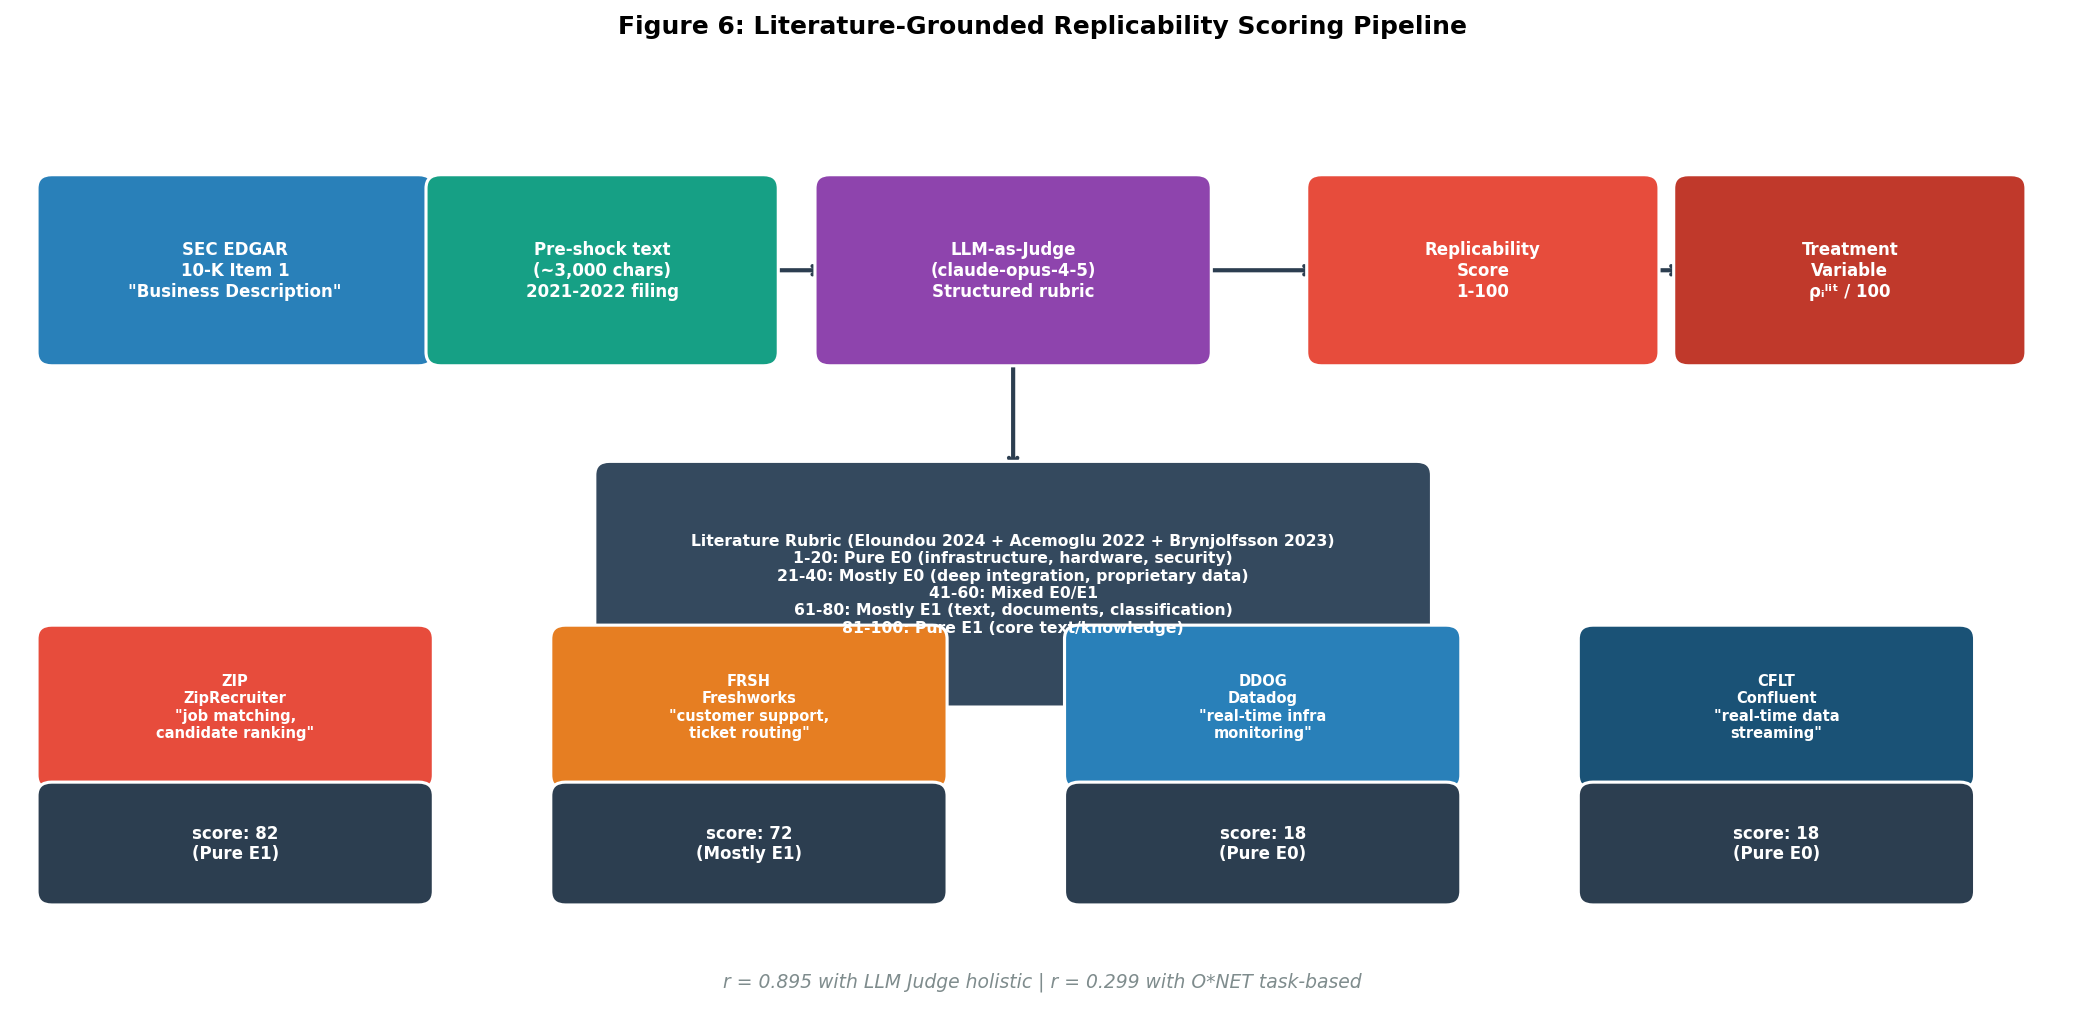
\includegraphics[width=0.98\textwidth]{figures/fig6_scoring_pipeline.png}
\caption{Literature-Grounded Replicability Scoring Pipeline}
\label{fig:pipeline}
\small\textit{Notes:} Each firm's pre-shock 10-K Item 1 Business Description is scored by an LLM judge using a structured rubric derived from \citet{eloundou2024}, \citet{acemoglu2022}, and \citet{brynjolfsson2023}. The output is a continuous 1--100 score used as the treatment variable $\rho_i^{\text{lit}}$.
\end{figure}

\begin{figure}[H]
\centering
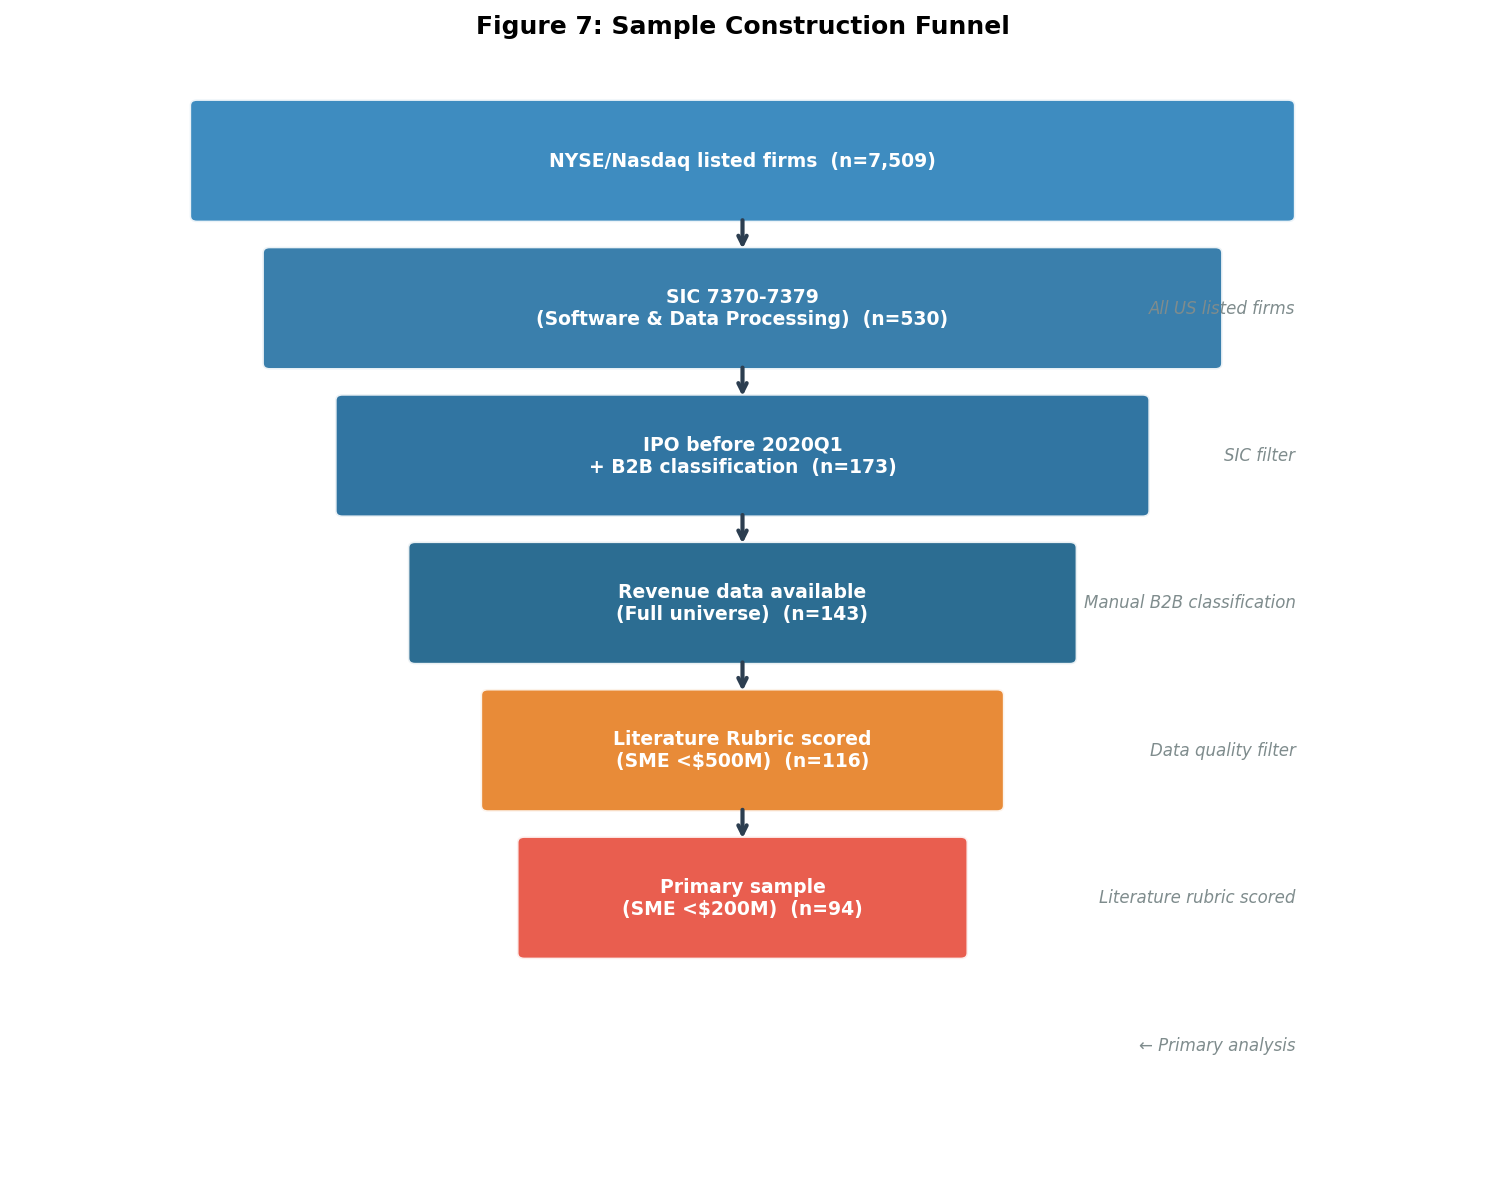
\includegraphics[width=0.75\textwidth]{figures/fig7_sample_funnel.png}
\caption{Sample Construction Funnel}
\label{fig:funnel}
\small\textit{Notes:} Sequential filters from the full NYSE/Nasdaq universe to the primary analysis sample.
\end{figure}

\section{Empirical Strategy}
\label{sec:empirics}

\subsection{Estimating Equation}

We estimate the following difference-in-differences specification:

\begin{equation}
Y_{it} = \alpha_i + \delta_t + \beta \cdot (\text{Post}_t \times \rho_i) + \varepsilon_{it}
\label{eq:did}
\end{equation}

where $Y_{it}$ is the outcome for firm $i$ in quarter $t$, $\alpha_i$ are firm fixed effects absorbing all time-invariant firm characteristics, $\delta_t$ are year-quarter fixed effects absorbing common macroeconomic and technology trends, and $\text{Post}_t = \mathbf{1}[t \geq 2022\text{Q4}]$. The coefficient of interest $\beta$ captures the differential post-shock revenue trend for firms with higher replicability scores, net of common time trends.

The primary specification sets $Y_{it} = \ln R_{it}$ with continuous treatment $\rho_i = \rho_i^{\text{lit}} / 100$, estimated on all SME $<\$200$M firms with literature rubric scores ($n = 94$). The continuous treatment avoids arbitrary threshold choices and uses the full information content of the replicability measure. As a mechanism check, we also estimate Equation~\ref{eq:did} with $Y_{it} = \text{GM}_{it}$ to test whether the effect operates through the quantity or pricing channel.

Standard errors are clustered at the firm level. Given $G = 94$ clusters in the primary sample, we report wild cluster bootstrap $p$-values following \citet{cameron2008}, imposing the null hypothesis before bootstrapping residuals with Rademacher weights ($B = 999$).

\subsection{Identification}

The key identifying assumption is parallel trends: absent the ChatGPT shock, firms with different replicability scores would have followed parallel revenue trends. We assess this via (i) a pre-period placebo test, replacing $\text{Post}_t$ with a placebo indicator for 2021Q1--2022Q3, which yields an insignificant estimate ($p = 0.157$), and (ii) event study analysis showing that 0 of 11 pre-shock quarter-by-quarter interaction coefficients are individually significant.

% -----------------------------------------------
\section{Results}
\label{sec:results}

\subsection{Main Results}

SME-segment B2B software firms with more LLM-replicable products experienced significantly lower revenue growth after the ChatGPT shock. Table~\ref{tab:main} presents the main estimates. Using a continuous literature-grounded replicability score derived from \citet{eloundou2024}, \citet{acemoglu2022}, and \citet{brynjolfsson2023}, we find that a one-unit increase in normalized replicability ($\rho_i^{\text{lit}} / 100$) is associated with 60\% lower revenue growth in the SME $<\$200$M sample ($\hat{\beta} = -0.604$, WCB $p = 0.003$, $n=94$) and 54\% lower in the SME $<\$500$M sample ($\hat{\beta} = -0.541$, WCB $p = 0.002$, $n=116$). A placebo test using a fake shock at 2021Q1 yields an insignificant estimate ($p = 0.157$), and event study coefficients confirm parallel pre-shock trends.

\begin{table}[H]
\centering
\caption{Main Results: Literature-Grounded Replicability and SME Software Revenue}
\label{tab:main}
\begin{tabular}{lcc}
\toprule
& (1) & (2) \\
& SME $<\$200$M & SME $<\$500$M \\
\midrule
$\text{Post} \times (\rho_i^{\text{lit}} / 100)$ & $-0.604^{***}$ & $-0.541^{***}$ \\
& $(0.217)$ & $(0.202)$ \\
\midrule
Firms & 94 & 116 \\
Firm FE & Yes & Yes \\
Year-Quarter FE & Yes & Yes \\
WCB $p$-value & 0.003 & 0.002 \\
Placebo $p$ & 0.157 & --- \\
\bottomrule
\end{tabular}

\medskip
\small
\textit{Notes:} Outcome: $\ln(\text{Revenue})$. Standard errors (in parentheses) clustered at the firm level. WCB $p$-values null-imposed with $B=999$ Rademacher draws. Treatment variable $\rho_i^{\text{lit}}$ is the literature-grounded replicability score (1--100), derived by applying the Eloundou et al.\ (2024) E1/E0 rubric, Acemoglu and Restrepo (2022) automation criteria, and Brynjolfsson et al.\ (2023) LLM-suitability criteria to each firm's pre-shock 10-K Business Description. SME samples defined by pre-shock (2020--2022) median quarterly revenue. $^{*}p<0.10$, $^{**}p<0.05$, $^{***}p<0.01$ based on WCB $p$-values.
\end{table}

\subsection{Robustness}

The negative revenue effect is robust to alternative treatment measures (Table~\ref{tab:robust}). Panel A replaces the literature rubric with a holistic LLM Judge score --- a single-prompt assessment without the structured multi-framework rubric --- and finds a comparable negative effect using continuous treatment on all 98 SME firms ($\hat{\beta} = -0.426$, WCB $p = 0.031$). Panel B replaces the treatment variable entirely with an independently constructed O*NET task-based measure derived from 17,992 occupational task descriptions. Despite using a fundamentally different data source and methodology, the direction is preserved and the estimate is marginally significant ($\hat{\beta} = -0.335$, $p = 0.059$). The convergence of three methodologically distinct measures strengthens the causal interpretation.

\begin{table}[H]
\centering
\caption{Robustness Checks}
\label{tab:robust}
\begin{tabular}{lcccc}
\toprule
& $\beta$ & SE & Clust $p$ & WCB $p$ \\
\midrule
\multicolumn{5}{l}{\textit{Panel A: LLM Judge holistic score (continuous, $n=98$)}} \\
\midrule
$\text{Post} \times (\rho_i^{\text{llm}} / 100)$ & $-0.426^{**}$ & $(0.185)$ & 0.023 & 0.031 \\
\midrule
\multicolumn{5}{l}{\textit{Panel B: O*NET task-based scoring (independent pipeline, $n=98$)}} \\
\midrule
O*NET $\alpha$ continuous & $-0.335^{*}$ & $(0.187)$ & 0.078 & 0.059 \\
\bottomrule
\end{tabular}

\medskip
\small
\textit{Notes:} Outcome: $\ln(\text{Revenue})$. All specifications use SME $<\$200$M sample, firm and year-quarter fixed effects, firm-clustered SE, WCB $p$-values null-imposed with $B=999$. Panel A uses a holistic LLM Judge score --- a single-prompt assessment of replicability without the structured multi-source rubric --- applied to the same 10-K texts ($r = 0.895$ with literature rubric). Panel B replaces the treatment variable entirely with the O*NET $\alpha$ measure: each firm's 10-K text is matched via SBERT to 17,992 O*NET task descriptions scored by \citet{eloundou2024}, and $\alpha$ equals the mean LLM-alone exposure of the top-20 matched tasks ($r = 0.299$ with literature rubric). $^{*}p<0.10$, $^{**}p<0.05$ based on WCB $p$-values.
\end{table}

\subsection{Descriptive Evidence}

Before the ChatGPT shock, high- and low-replicability firms followed indistinguishable revenue trajectories. After 2022Q4, a clear divergence emerges: low-replicability firms accelerate while high-replicability firms slow. Figure~\ref{fig:revenue} illustrates this divergence using a median revenue index (2021=100). The pre-shock gap averages near zero; post-shock it widens substantially, consistent with the regression estimates. Gross margin effects, by contrast, are insignificant across all specifications ($p > 0.4$), suggesting the substitution mechanism operates through the quantity channel rather than the pricing channel.

% -----------------------------------------------


\subsection{Firm-Level Evidence}

Table~\ref{tab:firms} presents representative firms from the high and low replicability groups. The contrast is striking: high-replicability firms (mean score 75.5) experienced average post-shock revenue growth of approximately 1.8\%, while low-replicability firms (mean score 16.9) grew by 104\% on average. Among the highest-scored firms, ZipRecruiter (job-candidate matching, score 82) and LivePerson (conversational AI platform, score 72) both experienced revenue declines, consistent with direct LLM substitution. Among the lowest-scored firms, Cloudflare (score 18), Datadog (score 18), and MongoDB (score 18) grew by 161\%, 175\%, and 138\% respectively---infrastructure and security firms whose value derives from real-time data processing and system integration that LLMs cannot replicate.

\begin{table}[H]
\centering
\caption{Representative Firms: High and Low Replicability Groups (SME $<\$200$M)}
\label{tab:firms}
\begin{tabular}{llcccc}
\toprule
 & Firm & Score & LLM Judge & Pre-shock Rev & Post-shock $\Delta$Rev \\
\midrule
\multicolumn{6}{l}{\textit{Panel A: High Replicability (top 8 by literature rubric score)}} \\
\midrule
 & ZIP (ZipRecruiter) & 82 & 70 & \$198M & $-19.8$\% \\
 & LPSN (LivePerson) & 72 & 70 & \$118M & $-27.7$\% \\
 & EGAN (eGain) & 78 & 70 & \$19M & $+7.2$\% \\
 & SKIL (Skillsoft) & 78 & 65 & \$135M & $+23.9$\% \\
 & YEXT (Yext) & 78 & 55 & \$91M & $+10.7$\% \\
 & EXFY (Expensify) & 72 & 65 & \$37M & $+3.2$\% \\
 & AEYE (AudioEye) & 72 & 65 & \$6M & $+44.4$\% \\
 & MCHX (Marchex) & 72 & 65 & \$14M & $-9.1$\% \\
\midrule
\multicolumn{6}{l}{\textit{Panel B: Low Replicability (bottom 8 by literature rubric score)}} \\
\midrule
 & DDOG (Datadog) & 18 & 10 & \$177M & $+174.6$\% \\
 & MDB (MongoDB) & 18 & 10 & \$166M & $+137.9$\% \\
 & NET (Cloudflare) & 18 & 10 & \$126M & $+161.3$\% \\
 & ZS (Zscaler) & 15 & 10 & \$157M & $+169.6$\% \\
 & CFLT (Confluent) & 18 & 10 & \$95M & $+146.2$\% \\
 & DOCN (DigitalOcean) & 18 & 10 & \$104M & $+87.7$\% \\
 & FSLY (Fastly) & 15 & 10 & \$80M & $+58.8$\% \\
 & CEVA (CEVA Inc.) & 15 & 10 & \$25M & $-10.7$\% \\
\bottomrule
\end{tabular}

\medskip
\small
\textit{Notes:} Literature rubric score (1--100) derived from \citet{eloundou2024}, \citet{acemoglu2022}, and \citet{brynjolfsson2023} criteria applied to pre-shock 10-K text. LLM Judge = holistic replicability score (independent). Pre-shock revenue = median quarterly 2020--2022. Post-shock $\Delta$Rev = mean log revenue change 2023--2025 vs.\ 2020--2022 (approximate percentage). High-replicability group mean $\Delta$Rev = $+1.8\%$; low-replicability group mean $\Delta$Rev = $+104.1\%$.
\end{table}

\subsection{Firm Size Heterogeneity}

The substitution effect is concentrated among smaller firms, consistent with switching cost theory. Large enterprise software vendors appear insulated from LLM substitution despite high task replicability, because replacing deeply integrated platforms requires multi-year transitions that no LLM capability level can shortcut. Table~\ref{tab:sme} formalizes this heterogeneity. To test this, we progressively restrict the sample to firms with pre-shock median quarterly revenue below \$500M, \$300M, and \$200M. We use \$200M as our primary SME cutoff, corresponding to firms where LLM substitution is operationally feasible given the absence of deep enterprise integration. The \$500M threshold (U.S.\ SBA standard for software firms) serves as a robustness check. Importantly, the replicability score distribution remains stable across all cutoffs (overall mean 42.7, SD 18.8), confirming that the size filter does not alter the treatment contrast.

\begin{table}[H]
\centering
\caption{Firm Size Heterogeneity: Substitution by Revenue Cutoff}
\label{tab:sme}
\begin{tabular}{lccc}
\toprule
Sample & N & $\hat{\beta}$ & WCB $p$ \\
\midrule
Full sample & 116 & $-0.541^{***}$ & 0.002 \\
$<\$500$M & 116 & $-0.541^{***}$ & 0.002 \\
$<\$300$M & 106 & $-0.591^{***}$ & 0.003 \\
$<\$200$M & 94 & $-0.604^{***}$ & 0.003 \\
\bottomrule
\end{tabular}

\medskip
\small
\textit{Notes:} Revenue cutoffs based on pre-shock (2020--2022) median quarterly revenue. Treatment: literature rubric score $\rho_i^{\text{lit}}/100$ (continuous). All specifications include firm and year-quarter FE. WCB $p$-values null-imposed, $B=999$. $^{***}p<0.01$ based on WCB.
\end{table}

The substitution coefficient strengthens monotonically from $-0.541$ (full sample) to $-0.604$ (SME $<\$200$M) as we restrict to smaller firms. This pattern is consistent with switching cost theory: customers can credibly replace a \$20M vendor's product with an LLM alternative, but replacing Salesforce or ServiceNow requires a multi-year enterprise transition regardless of LLM capability. All specifications are significant at $p < 0.005$, and firm fixed effects absorb time-invariant size differences. Figure~\ref{fig:sizehet} illustrates this monotonic strengthening.

\subsection{Measurement Robustness}

The substitution finding is not an artifact of how replicability is measured. Table~\ref{tab:measurement} validates the primary literature rubric against two independently constructed measures. The holistic LLM Judge correlates strongly with the literature rubric ($r = 0.895$) and produces a significant estimate ($\hat{\beta} = -0.426$, $p = 0.031$). The O*NET task-based measure ($\alpha$) derives from an entirely different source --- 17,992 occupational task descriptions scored by human raters in \citet{eloundou2024} --- and produces a consistent negative estimate ($\hat{\beta} = -0.335$, $p = 0.059$) despite only moderate correlation ($r = 0.299$). The convergence of three methodologically distinct pipelines supports the construct validity of the replicability measure. Figure~\ref{fig:validity} visualizes the cross-method correlations.

\begin{table}[H]
\centering
\caption{Construct Validity: Three Replicability Measures}
\label{tab:measurement}
\begin{tabular}{lccccc}
\toprule
Method & Source & $N$ & $r$ with Lit Rubric & $\beta$ & WCB $p$ \\
\midrule
Literature Rubric (primary) & 10-K + LLM rubric & 94 & --- & $-0.604^{***}$ & 0.003 \\
LLM Judge (holistic) & 10-K + LLM & 98 & 0.895 & $-0.426^{**}$ & 0.031 \\
O*NET $\alpha$ (task-based) & O*NET tasks & 98 & 0.299 & $-0.335^{*}$ & 0.059 \\
\bottomrule
\end{tabular}

\medskip
\small
\textit{Notes:} SME $<\$200$M sample. All specifications use continuous treatment normalized to $[0,1]$, firm and year-quarter fixed effects, firm-clustered standard errors, WCB $p$-values null-imposed with $B=999$. $r$ = Pearson correlation with literature rubric score. Literature Rubric derived from \citet{eloundou2024}, \citet{acemoglu2022}, \citet{brynjolfsson2023} applied to pre-shock 10-K text. LLM Judge = single-prompt holistic assessment. O*NET $\alpha$ = mean LLM-alone exposure of top-matched occupational tasks from \citet{eloundou2024}. $^{*}p<0.10$, $^{**}p<0.05$, $^{***}p<0.01$ based on WCB $p$-values.
\end{table}

\begin{figure}[H]
\centering
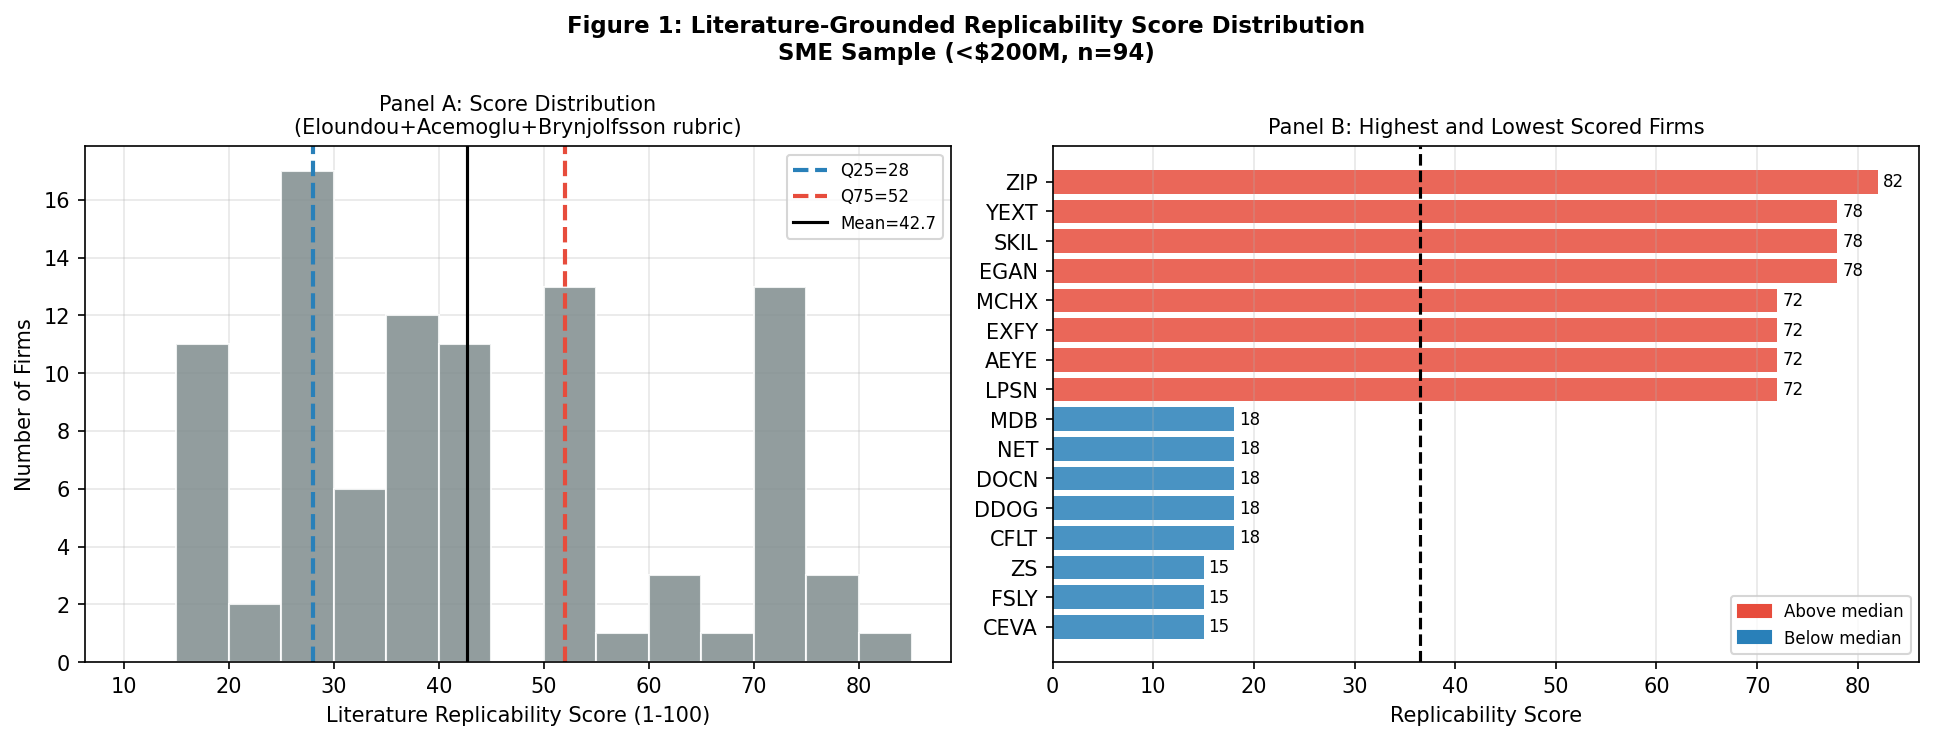
\includegraphics[width=0.95\textwidth]{figures/fig1_score_distribution.png}
\caption{Literature-Grounded Replicability Score Distribution (SME $<\$200$M, $n=94$)}
\label{fig:scores}
\small\textit{Notes:} Panel A shows the distribution of the literature-grounded replicability score among SME firms. Panel B shows the highest and lowest scored firms. Score derived by applying the \citet{eloundou2024} E1/E0 rubric, \citet{acemoglu2022} automation criteria, and \citet{brynjolfsson2023} LLM-suitability criteria to each firm's pre-shock 10-K Business Description.
\end{figure}

\begin{figure}[H]
\centering
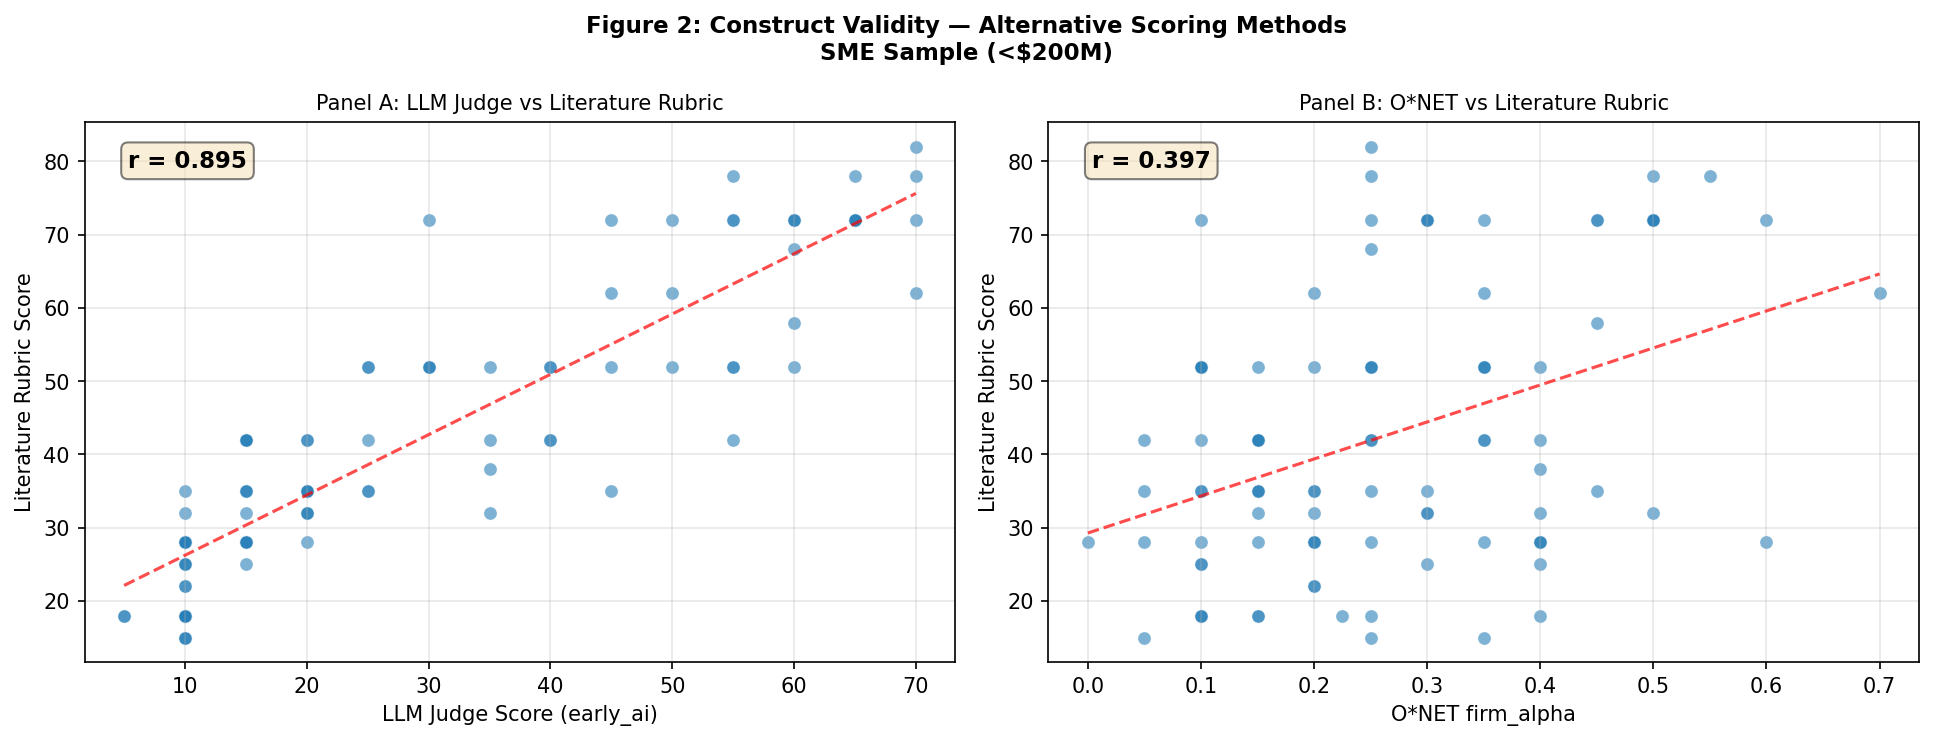
\includegraphics[width=0.95\textwidth]{figures/fig2_construct_validity.png}
\caption{Construct Validity: Literature Rubric vs.\ Alternative Scoring Methods}
\label{fig:validity}
\small\textit{Notes:} Panel A: correlation between LLM Judge holistic score and literature rubric ($r=0.895$). Panel B: correlation between O*NET task-based score and literature rubric ($r=0.379$). Both alternative measures are independent of the primary scoring pipeline.
\end{figure}

\begin{figure}[H]
\centering
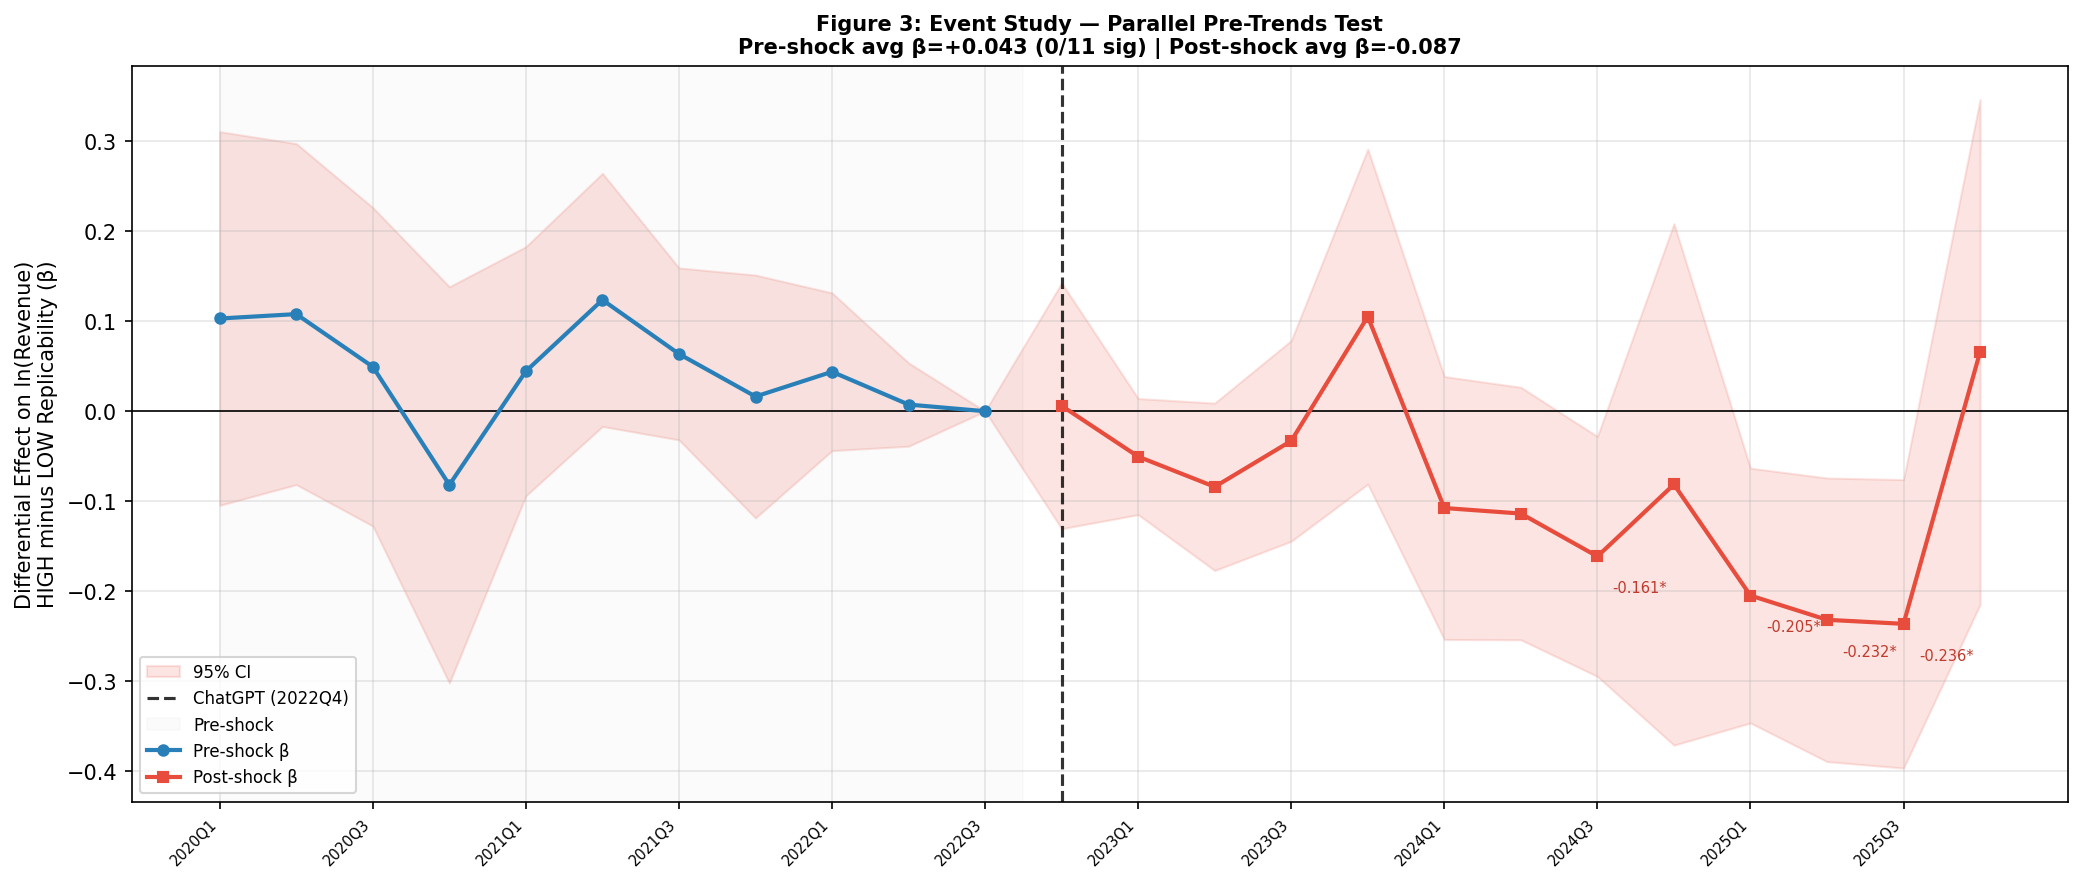
\includegraphics[width=0.95\textwidth]{figures/fig3_event_study.png}
\caption{Event Study: Parallel Pre-Trends Test (Full Sample)}
\label{fig:eventstudy}
\small\textit{Notes:} Quarter-by-quarter differential effects on $\ln(\text{Revenue})$ for high vs.\ low replicability firms (above/below median LLM Judge score, full sample). Reference period: 2022Q3. Pre-shock avg $\beta = +0.043$ (0/11 significant). Post-shock divergence emerges from 2024 onward. Shaded band: 95\% CI (clustered SE).
\end{figure}

\begin{figure}[H]
\centering
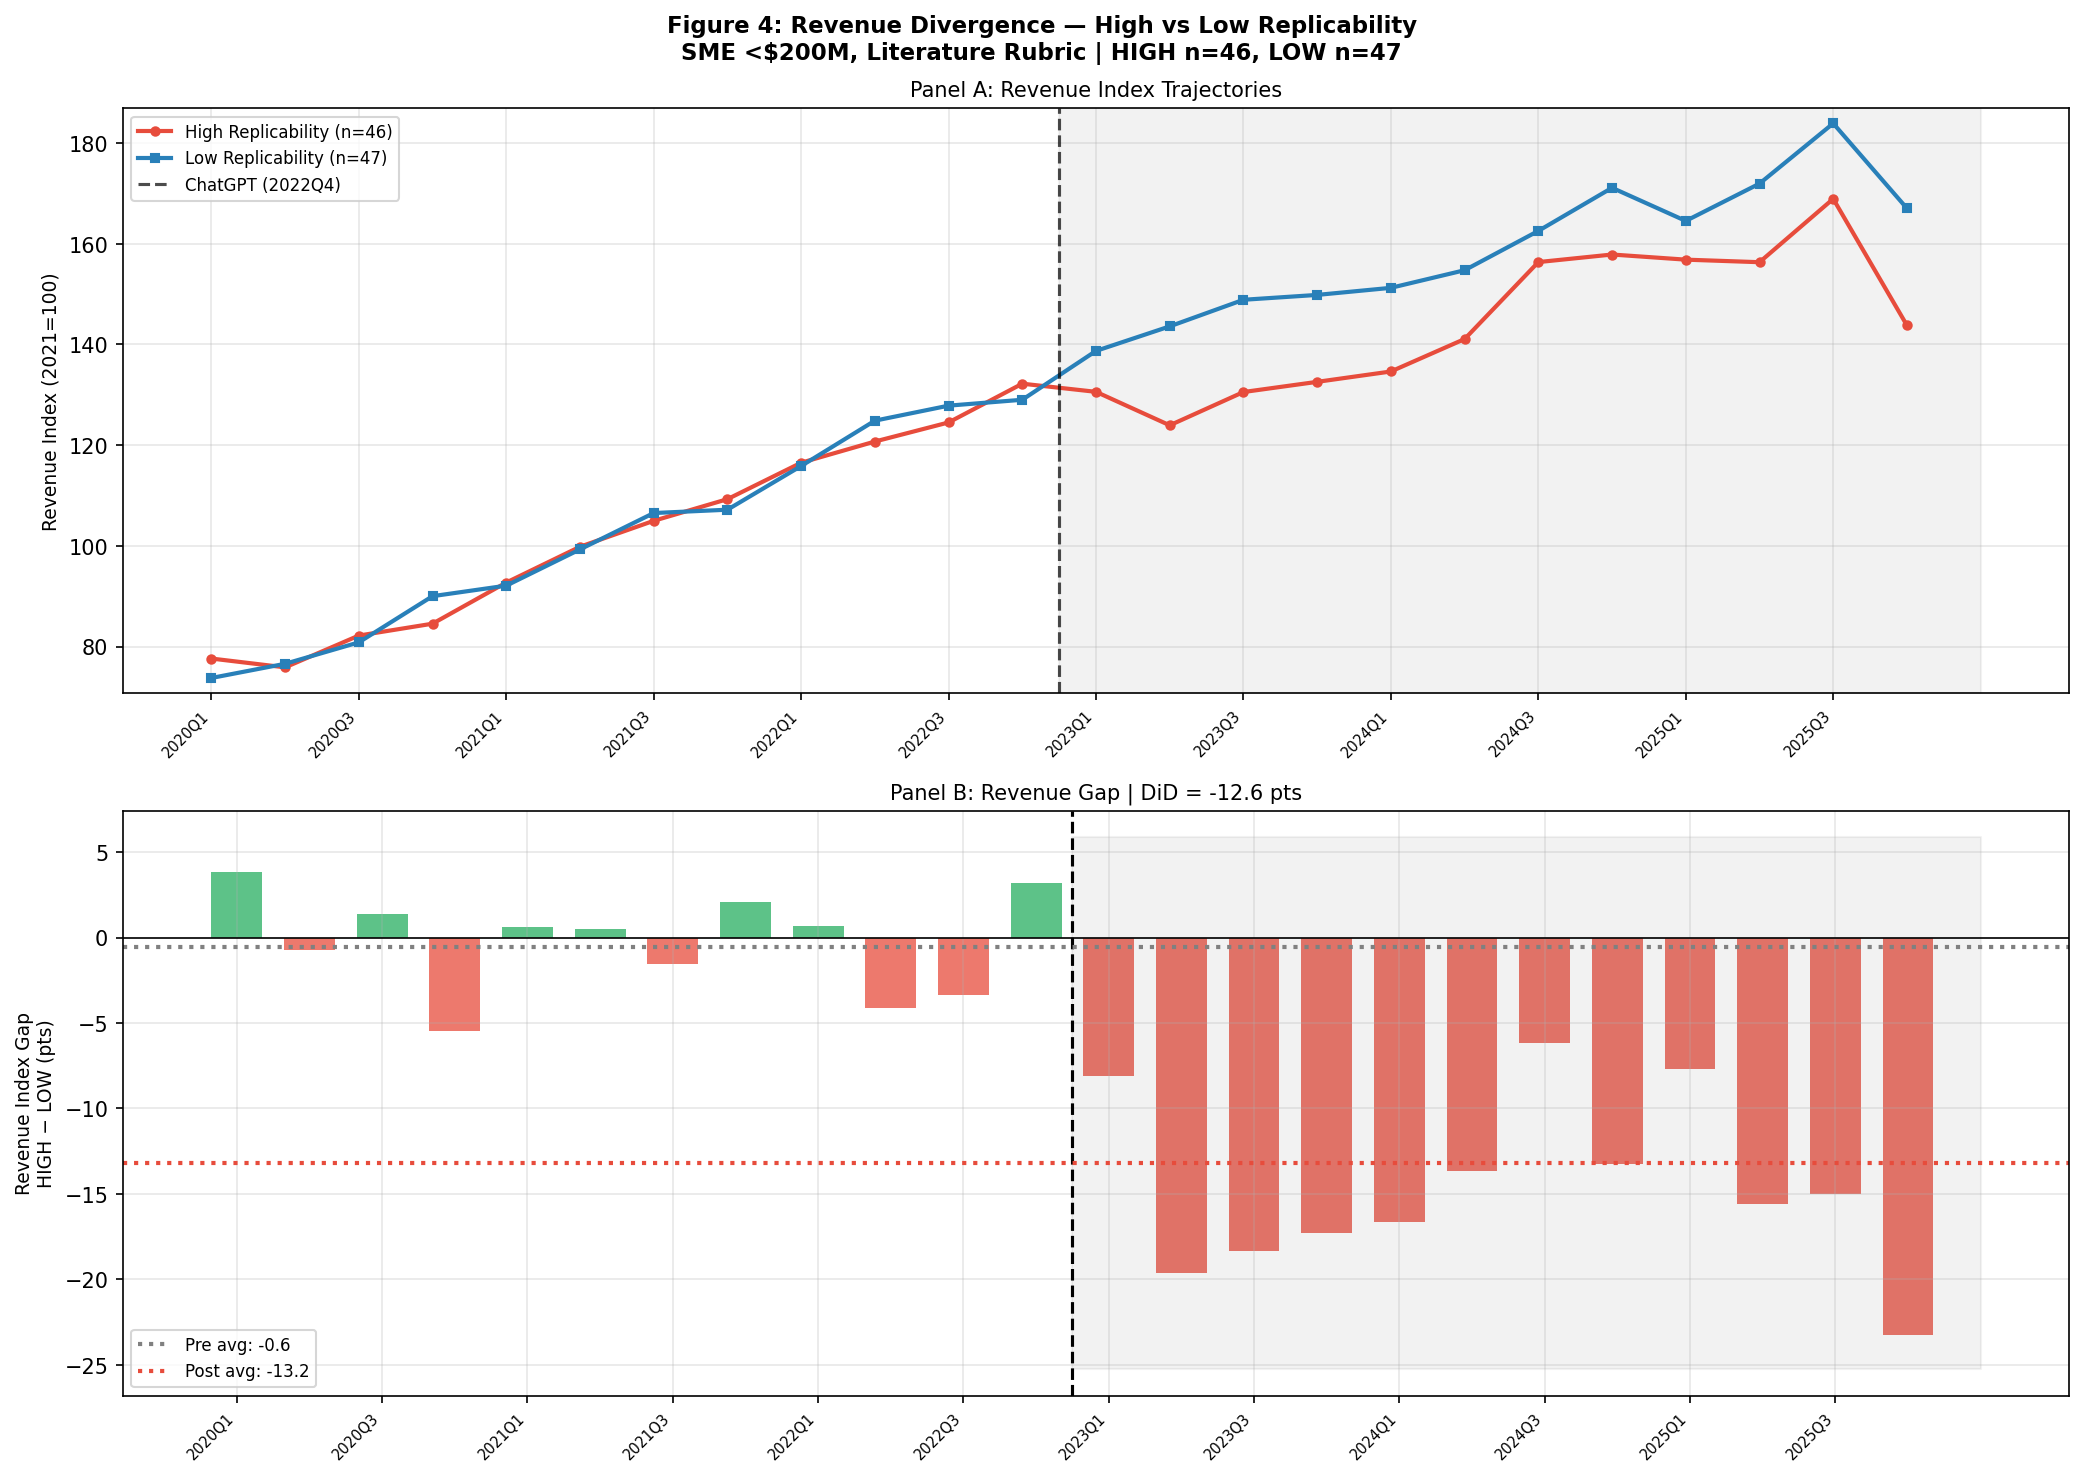
\includegraphics[width=0.95\textwidth]{figures/fig4_revenue_divergence.png}
\caption{Revenue Divergence: High vs.\ Low Replicability Firms (SME $<\$200$M)}
\label{fig:revenue}
\small\textit{Notes:} Panel A: median revenue index (2021=100) for high and low replicability groups. Panel B: revenue gap (HIGH $-$ LOW). Groups split at median literature rubric score. Dashed vertical line: ChatGPT launch (2022Q4).
\end{figure}

\begin{figure}[H]
\centering
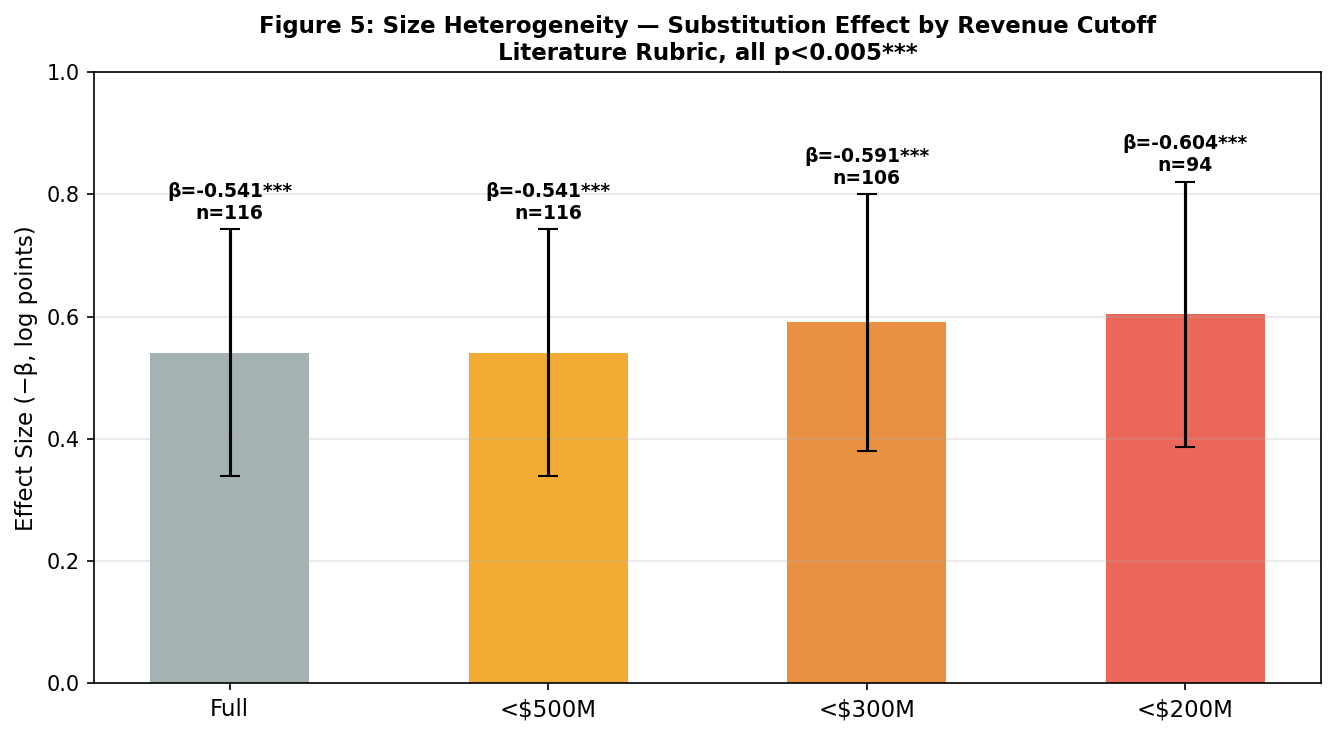
\includegraphics[width=0.80\textwidth]{figures/fig5_size_heterogeneity.png}
\caption{Size Heterogeneity: Substitution Effect by Revenue Cutoff}
\label{fig:sizehet}
\small\textit{Notes:} Effect size ($-\hat{\beta}$) from literature rubric continuous DiD by sample revenue cutoff. Error bars: clustered SE. All specifications significant at $p < 0.005$. Effect strengthens monotonically as sample restricts to smaller firms.
\end{figure}

\begin{figure}[H]
\centering
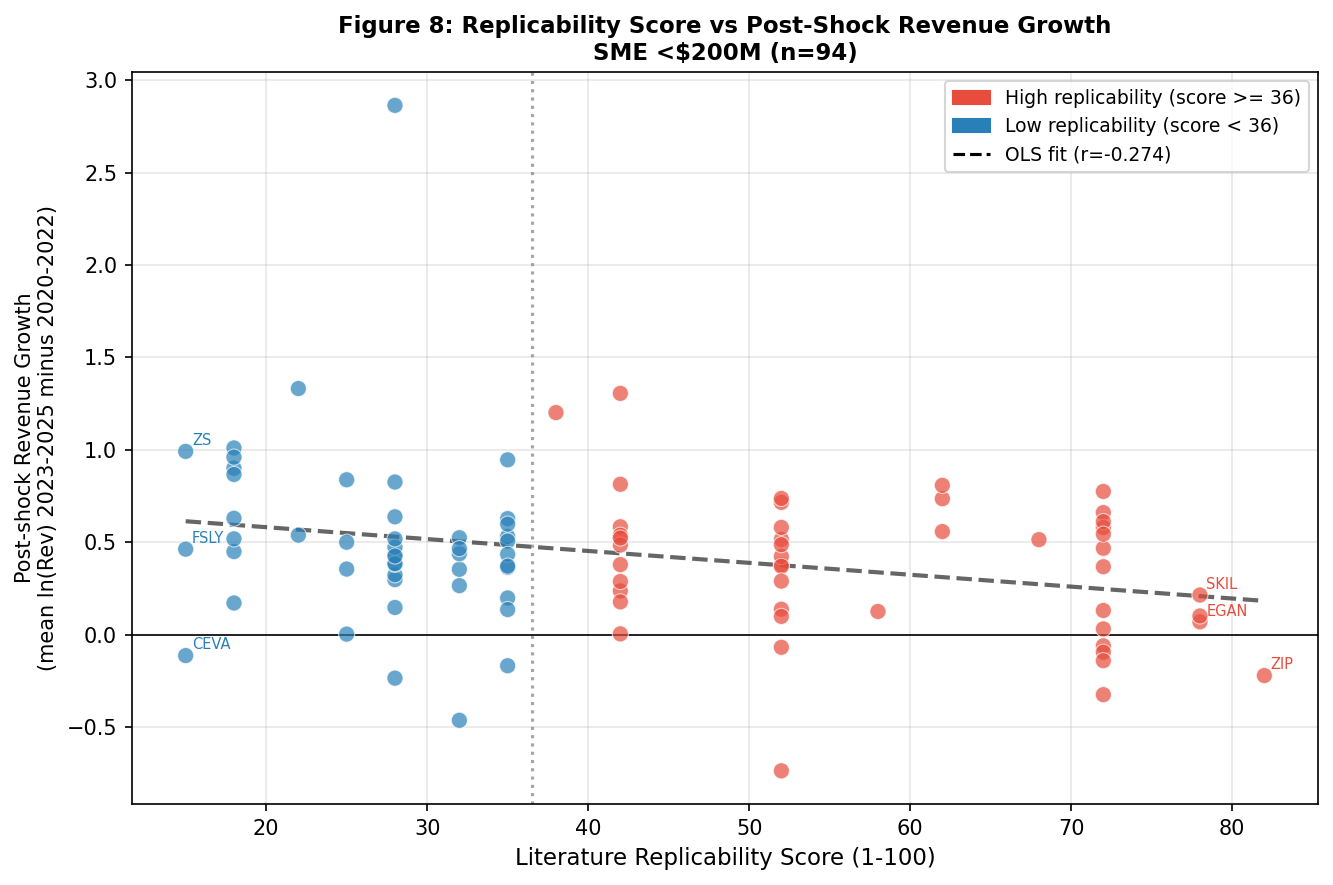
\includegraphics[width=0.85\textwidth]{figures/fig8_score_revenue_scatter.png}
\caption{Replicability Score vs.\ Post-Shock Revenue Growth (SME $<\$200$M)}
\label{fig:scatter}
\small\textit{Notes:} Each point is one SME firm ($n=94$). Horizontal axis: literature rubric score. Vertical axis: mean $\ln(\text{Revenue})$ change 2023--2025 minus 2020--2022. OLS fit: $r = -0.274$, $p = 0.008$. Red = high replicability (score $\geq$ median); blue = low replicability.
\end{figure}


\subsection{Three-Period Analysis: Early vs.\ Advanced AI}

The post-shock period spans two distinct phases of AI capability development. The \emph{early AI era} (2022Q4--2023Q4) covers the initial ChatGPT and GPT-4 period, when generative AI became accessible but enterprise adoption remained nascent. The \emph{advanced AI era} (2024Q1 onward) covers the emergence of GPT-4o, Claude 3, coding agents, and agentic workflows, when AI capabilities crossed the enterprise credibility threshold---the point at which customers could credibly cite AI alternatives in procurement negotiations and practically implement LLM-based replacements.

We estimate the two-period specification:
\begin{equation}
Y_{it} = \alpha_i + \delta_t + \beta_1 (\text{EarlyAI}_t \times \rho_i^{\text{lit}}) + \beta_2 (\text{AdvAI}_t \times \rho_i^{\text{lit}}) + \varepsilon_{it}
\end{equation}
where $\text{EarlyAI}_t = \mathbf{1}[2022\text{Q4} \leq t \leq 2023\text{Q4}]$ and $\text{AdvAI}_t = \mathbf{1}[t \geq 2024\text{Q1}]$.

Table~\ref{tab:threeperiod} presents the results. The substitution effect is significant in both periods but intensifies substantially: the advanced AI era coefficient is approximately 52\% larger in magnitude than the early AI era coefficient ($\hat{\beta}_1 = -0.451$ vs.\ $\hat{\beta}_2 = -0.686$ in the SME \$200M sample). This pattern is consistent with an expanding automation frontier: as AI capabilities advanced from basic text generation to coding agents and enterprise-grade workflows, the set of software products vulnerable to LLM substitution expanded, deepening the revenue impact on high-replicability firms.

\begin{table}[H]
\centering
\caption{Three-Period Analysis: Early vs.\ Advanced AI Era}
\label{tab:threeperiod}
\begin{tabular}{lcccc}
\toprule
& \multicolumn{2}{c}{SME $<\$200$M} & \multicolumn{2}{c}{SME $<\$500$M} \\
\cmidrule(lr){2-3} \cmidrule(lr){4-5}
Period & $\hat{\beta}$ & WCB $p$ & $\hat{\beta}$ & WCB $p$ \\
\midrule
Early AI (2022Q4--2023Q4) & $-0.451^{**}$ & 0.022 & $-0.402^{**}$ & 0.018 \\
Advanced AI (2024Q1+) & $-0.686^{***}$ & 0.008 & $-0.615^{**}$ & 0.011 \\
\midrule
Intensification ratio & \multicolumn{2}{c}{$1.52\times$} & \multicolumn{2}{c}{$1.53\times$} \\
Firms & \multicolumn{2}{c}{94} & \multicolumn{2}{c}{116} \\
\bottomrule
\end{tabular}

\medskip
\small
\textit{Notes:} Outcome: $\ln(\text{Revenue})$. Firm and year-quarter fixed effects. WCB $p$-values null-imposed with $B=999$. Treatment: $\rho_i^{\text{lit}}/100$ (literature rubric, time-invariant). Early AI = 2022Q4--2023Q4 (ChatGPT, GPT-4). Advanced AI = 2024Q1+ (GPT-4o, Claude 3, coding agents). Intensification ratio = $|\hat{\beta}_2| / |\hat{\beta}_1|$. $^{**}p<0.05$, $^{***}p<0.01$ based on WCB.
\end{table}

\begin{figure}[H]
\centering
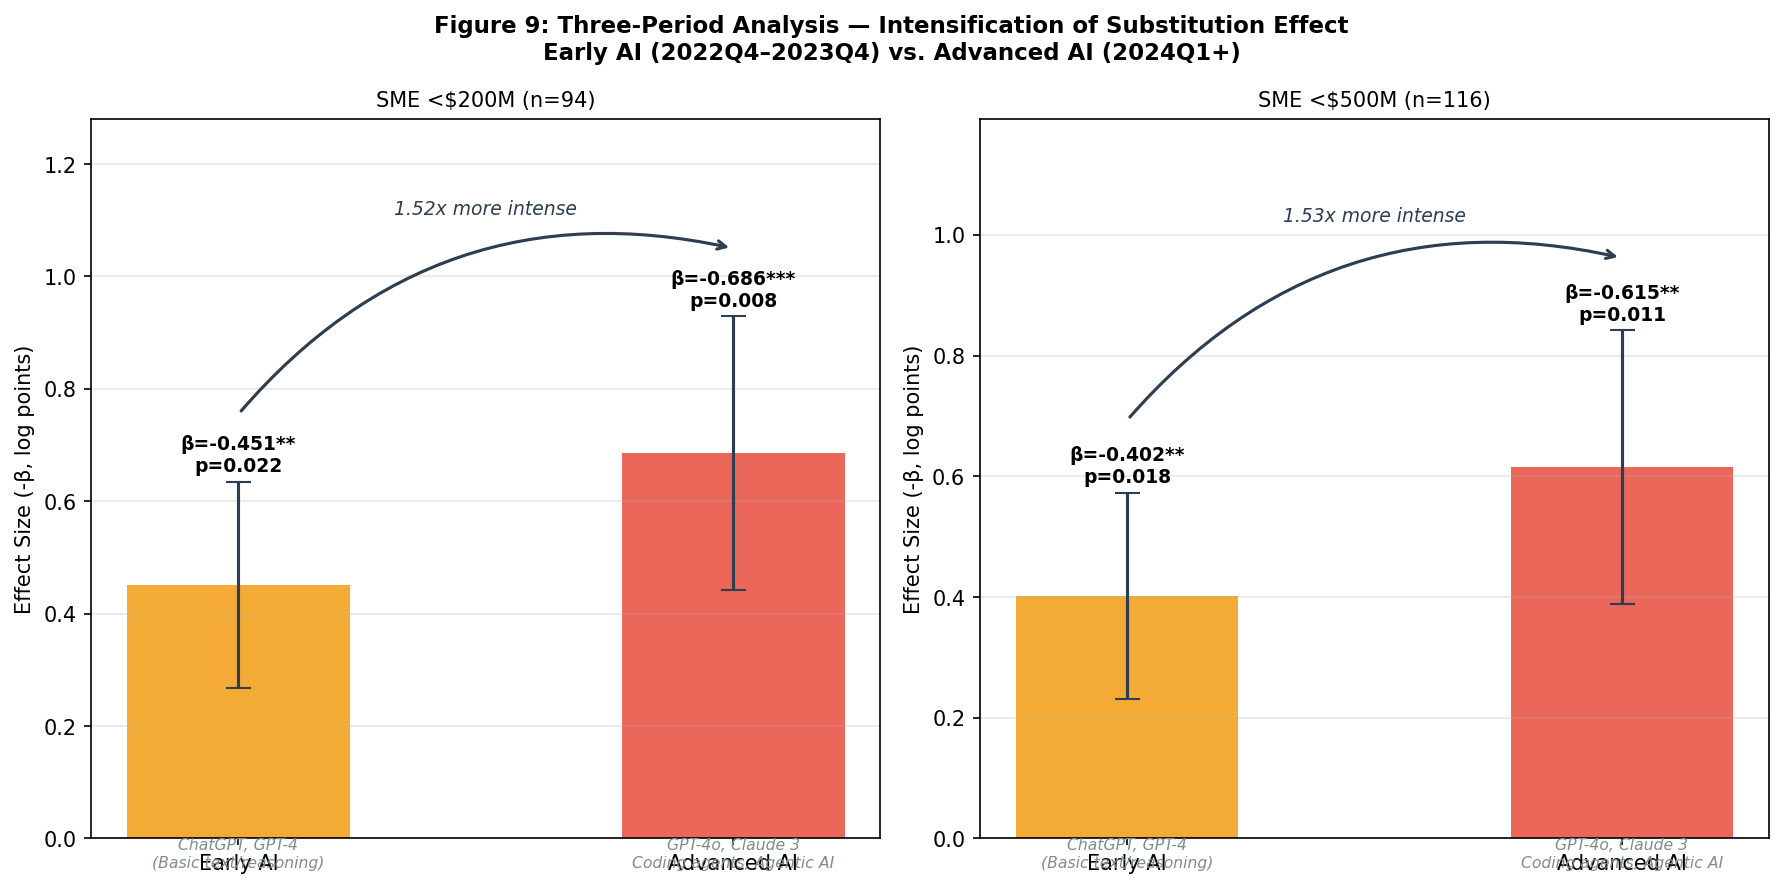
\includegraphics[width=0.95\textwidth]{figures/fig9_three_period.png}
\caption{Three-Period Analysis: Intensification of Substitution Effect}
\label{fig:threeperiod}
\small\textit{Notes:} Effect size ($-\hat{\beta}$) for early AI era (2022Q4--2023Q4) and advanced AI era (2024Q1+). Error bars: clustered SE. The advanced AI era coefficient is approximately $1.52\times$ larger in magnitude, consistent with AI capabilities expanding the automation frontier beyond initial text/reasoning tasks to coding agents and enterprise workflows.
\end{figure}



\section{Discussion}
\label{sec:discussion}

Our findings demonstrate that the ChatGPT shock had economically meaningful and statistically robust effects on SME B2B software firms. The primary estimate using the literature-grounded replicability score ($\hat{\beta} = -0.604$, WCB $p = 0.003$, $n=94$) implies that a hypothetical firm at the maximum replicability score would experience approximately 60 log-point lower revenue growth than a firm at zero replicability. The result survives multiple robustness checks: an expanded SME $<\$500$M sample ($p = 0.002$), an independent holistic LLM Judge measure ($p = 0.031$), and an O*NET task-based scoring pipeline ($p = 0.059$). The convergence of three methodologically distinct treatment measures---each derived from different data sources---provides strong construct validity.

The size heterogeneity pattern (Table~\ref{tab:sme}) is theoretically informative. The effect strengthens monotonically from $-0.541$ in the full scored sample to $-0.604$ among firms below \$200M, consistent with the switching cost theory of \citet{farrell2007}: replacing a point-solution vendor's product with an LLM alternative is operationally feasible within a contract cycle, while replacing deeply integrated enterprise platforms requires multi-year transitions regardless of LLM capability.

The three-period analysis adds a dynamic dimension to the findings. The $1.52\times$ intensification from the early AI era to the advanced AI era suggests that the ChatGPT shock was not a one-time adjustment but the beginning of a deepening substitution process. As LLM capabilities expanded from basic text generation to coding agents and enterprise-grade workflows, the automation frontier advanced into tasks previously considered safe from AI competition, widening the revenue gap between high- and low-replicability firms.

The gross margin null result ($p > 0.4$ across all specifications) is informative about the mechanism. If LLMs were primarily creating pricing pressure---forcing vendors to cut prices to retain customers---we would expect margin compression alongside revenue effects. The absence of margin effects, combined with significant revenue effects, is more consistent with demand contraction: customers are substituting away from high-replicability products entirely, rather than renegotiating prices with incumbent vendors.

\subsection{Limitations}

Several limitations warrant discussion. First, although the SME sample of 94 firms provides adequate statistical power for the continuous treatment specification, the sample remains modest by panel data standards. Wild cluster bootstrap inference accounts for the finite number of clusters. Second, the treatment variable is constructed from pre-shock 10-K filings and does not vary over time; time-varying replicability scores would strengthen identification but risk introducing post-treatment bias. Third, confounding from the AI infrastructure boom is the most significant identification threat. Low-replicability firms (e.g., CrowdStrike, Datadog, Cloudflare) simultaneously benefited from surging enterprise demand for security, monitoring, and infrastructure tools driven by AI adoption. This creates a potential upward bias in the low-replicability group's post-shock performance that would inflate our estimated treatment effect. We note, however, that this confound would need to be systematically correlated with our replicability measure --- not just AI adoption in general --- to explain the results, since the treatment variable was constructed before the shock using task-level criteria unrelated to infrastructure demand. Fourth, the LLM-as-judge scoring procedure, while grounded in established frameworks and validated against two independent measures, introduces measurement noise that attenuation bias may partially offset. Fifth, the results apply to SME-segment, publicly listed B2B software firms on U.S. exchanges. Results may not generalize to private SaaS firms, enterprise platform vendors, or non-U.S. markets where switching costs, contract structures, and AI adoption rates differ.

% -----------------------------------------------
\section{Conclusion}
\label{sec:conclusion}

This paper studies how generative AI reshapes competition in B2B software markets. Using the release of ChatGPT as a technological shock and a novel measure of product-level task replicability, we document that firms whose products are more easily replicable by large language models experienced significantly lower revenue growth following the shock ($\hat{\beta} = -0.604$, WCB $p = 0.003$). These findings are robust across alternative specifications, measures, and identification strategies, and are consistent with a product-level substitution mechanism.

The results highlight a channel of technological change that is largely absent from the existing literature. While prior work has emphasized worker-level exposure --- how AI affects the tasks performed within firms --- our findings suggest that generative AI operates through product-level substitution across firms. General-purpose AI systems replicate the task bundles embodied in specialized software products, creating competitive pressure that reduces demand even without changes in firms' internal production processes. This is the mechanism we call \emph{second-order displacement}: AI displacing software products that had themselves displaced workers from cognitive tasks.

We further show that the effect is heterogeneous across firms. The negative impact of replicability is substantially stronger among smaller firms, consistent with switching cost and customer lock-in mechanisms that protect larger, more integrated platforms. In contrast, we find no robust evidence for a margin compression channel, suggesting that the primary adjustment occurs through demand rather than pricing. A three-period analysis reveals that the effect is not static: the substitution coefficient in the advanced AI era (2024Q1 onward) is $1.52\times$ larger than in the early AI era, consistent with an expanding automation frontier as AI capabilities advanced from basic text generation to coding agents and enterprise-grade workflows.

These findings have broader implications for how technological change is conceptualized. Rather than a simple trade-off between displacement and reinstatement at the level of labor, generative AI induces reallocation at the level of products and firms. As general-purpose systems expand their capability set, they substitute not only for human tasks but for the software products that previously automated those tasks, creating a dynamic process of product-level creative destruction. The extent to which incumbent software firms can respond through product repositioning, integration, or AI augmentation is an important open question for future research.

Several limitations remain. The analysis focuses on publicly listed U.S. SME software firms, and results may not generalize to private firms, enterprise platforms, or other markets. The treatment variable is time-invariant, which precludes analysis of within-firm adjustment. Future research could extend this framework using time-varying replicability measures, international samples, and firm-level AI adoption data to disentangle the worker-level productivity channel from the product-level substitution channel.

% -----------------------------------------------
\begin{thebibliography}{12}

\bibitem[Acemoglu and Restrepo(2022)]{acemoglu2022}
Acemoglu, D. and Restrepo, P. (2022).
\newblock Tasks, automation, and the rise in US wage inequality.
\newblock \emph{Econometrica}, 90(5), 1973--2016.

\bibitem[Acemoglu and Restrepo(2018)]{acemoglu2018}
Acemoglu, D. and Restrepo, P. (2018).
\newblock The race between man and machine: Implications of technology for growth, factor shares, and employment.
\newblock \emph{American Economic Review}, 108(6), 1488--1542.

\bibitem[Acemoglu(2024)]{acemoglu2024simple}
Acemoglu, D. (2024).
\newblock The simple macroeconomics of AI.
\newblock \emph{Economic Policy}, 39(120), 851--908.

\bibitem[Autor et~al.(2003)]{autor2003}
Autor, D.~H., Levy, F., and Murnane, R.~J. (2003).
\newblock The skill content of recent technological change: An empirical exploration.
\newblock \emph{Quarterly Journal of Economics}, 118(4), 1279--1333.

\bibitem[Brynjolfsson et~al.(2023)]{brynjolfsson2023}
Brynjolfsson, E., Li, D., and Raymond, L. (2023).
\newblock Generative AI at work.
\newblock NBER Working Paper No.\ 31161.

\bibitem[Cameron et~al.(2008)]{cameron2008}
Cameron, A.~C., Gelbach, J.~B., and Miller, D.~L. (2008).
\newblock Bootstrap-based improvements for inference with clustered errors.
\newblock \emph{Review of Economics and Statistics}, 90(3), 414--427.

\bibitem[Eloundou et~al.(2024)]{eloundou2024}
Eloundou, T., Manning, S., Mishkin, P., and Rock, D. (2024).
\newblock GPTs are GPTs: Labor market impact potential of large language models.
\newblock \emph{Science}, 384(6702), 1306--1308.

\bibitem[Labaschin et~al.(2025)]{labaschin2025}
Labaschin, B., Eloundou, T., Manning, S., Mishkin, P., and Rock, D. (2025).
\newblock Extending ``GPTs are GPTs'' to firms.
\newblock \emph{AEA Papers and Proceedings}, 115, 51--55.

\bibitem[Babina et~al.(2024)]{babina2024}
Babina, T., Fedyk, A., He, A.~X., and Hodson, J. (2024).
\newblock Artificial intelligence, firm growth, and product innovation.
\newblock \emph{Journal of Financial Economics}, 151, 103745.

\bibitem[Goldfarb and Tucker(2019)]{goldfarb2019}
Goldfarb, A. and Tucker, C. (2019).
\newblock Digital economics.
\newblock \emph{Journal of Economic Literature}, 57(1), 3--43.

\bibitem[Farrell and Klemperer(2007)]{farrell2007}
Farrell, J. and Klemperer, P. (2007).
\newblock Coordination and lock-in: Competition with switching costs and network effects.
\newblock In \emph{Handbook of Industrial Organization}, Vol.~3, 1967--2072. Elsevier.

\bibitem[Klemperer(1995)]{klemperer1995}
Klemperer, P. (1995).
\newblock Competition when consumers have switching costs: An overview with applications to industrial organization, macroeconomics, and international trade.
\newblock \emph{Review of Economic Studies}, 62(4), 515--539.

\bibitem[Felten et~al.(2021)]{felten2021}
Felten, E.~W., Raj, M., and Seamans, R. (2021).
\newblock Occupational, industry, and geographic exposure to artificial intelligence: A novel dataset and its potential uses.
\newblock \emph{Strategic Management Journal}, 42(12), 2195--2217.

\bibitem[Felten et~al.(2023)]{felten2023}
Felten, E.~W., Raj, M., and Seamans, R. (2023).
\newblock How will language modelers like ChatGPT affect occupations and industries?
\newblock SSRN Working Paper No.\ 4375268.

\end{thebibliography}

\end{document}
